\documentclass[a4paper,12pt,twoside,openright,final]{book}
\usepackage{cmap}                           % Поддержка поиска русских слов в PDF (pdflatex)
\usepackage[utf8]{inputenc}                 % Включаем поддержку UTF8
\usepackage[T2A]{fontenc}                   % Поддержка кириллицы в ЛаТеХ
\usepackage[english,russian]{babel}         % Включаем пакет для поддержки русского и английского языка с переносами.

\usepackage{amsmath}                        % Математическая библиотека
\usepackage{amsfonts}                       % Математическая библиотека: различные стили начертания формул (прямые, курсивы и т.п.).
\usepackage{amssymb}                        % Пакет amsfonts + несколько сотен дополнительных математических символов
\usepackage{amsthm}                         % Окружения "теорема", "лемма", и т.п.
\usepackage{amscd}                          % Поддержка коммутативных диаграмм
\usepackage{mathrsfs}                       % Математическая библиотека
\usepackage{mathtext}                       % Математическая библиотека
\usepackage{latexsym}                       % Математическая библиотека

\usepackage{hyperref}                       % Гиперссылки в электронной версии
\usepackage{vmargin}                        %
\usepackage{indentfirst}                    % Делать отступ в начале параграфа
\usepackage{enumerate}                      % Создание и автоматическая нумерация списков
\usepackage{tabularx}                       % Продвинутые таблицы
\usepackage{floatrow}                       % Продвинутое управление плавающими объектами
\usepackage{cite}                           % "Умные" библиографические ссылки (сортировка и сжатие)
\usepackage{multirow}                       % Возможность объединять строки в таблицах
\usepackage{showkeys}                       % Раскомментируйте, чтобы в документе были видны ссылки на литературу, рисунки и таблицы
\usepackage{tocvsec2}                       % Можно менять уровень вложенности в оглавлении

%\setpapersize{A4}
%\setmarginsrb{2cm}{1.5cm}{1cm}{1.5cm}{0pt}{0mm}{0pt}{13mm}

\setcounter{secnumdepth}{0}

\usepackage{graphicx}
\sloppy                                     % Борьба с залезанием строк на поля
\usepackage{nameref}                        % Ссылки на разделы

\usepackage{color}
\usepackage{listings}
\lstset{
  language=VHDL,
  numbers=left,
  firstnumber=0,
  backgroundcolor=\color{gray!10},
  inputencoding=utf8,
  extendedchars=false,
  keepspaces=true,
  breaklines=true,
  commentstyle=\color{green!60!black},
  % texcl=true
}

\usepackage{tikz}
\usetikzlibrary{arrows,calc,shapes.gates.logic.US}

\makeatletter
\def\lst@PlaceNumber{\ifnum\value{lstnumber}=0\else
  \llap{\normalfont\lst@numberstyle{\thelstnumber}\kern\lst@numbersep}\fi}
\makeatother

\usepackage{float}                          % Управление "плавающими" объектами
\floatstyle{plain} % optionally change the style of the new float
\newfloat{Code}{H}{myc}

\newcommand\exsect[1]{\textbf{\textit{\underline{#1}}}}

\title{Проектирование аппаратных схем ПЛИС средствами языка VHDL}

\date{}

\makeindex

\begin{document}
\frontmatter
\maketitle
\tableofcontents

\mainmatter
\chapter{Введение. Схемотехника комбинационных устройств.}


\emph{История развития интегральных схем (от транзистора до ПЛИС). Классификация современных ИС по методу соединения элементов. Общая архитектура ПЛИС. Конфигурационная память и возможность реконфигурации. Обзор семейства ПЛИС фирмы Xilinx. Применение ПЛИС в современном мире. Логические элементы в логике КМОП. Тристабильные элементы. Простые комбинационные элементы.}

\section{Вывод на консоль во время симуляции}

\chapter{Основы VHDL для синтеза и моделирования}

\emph{Введение в VHDL. Синтаксис и параллельная семантика. Объекты и конструкции. Типы данных. Логические и арифметические операторы языка. Синтезируемое подмножество языка VHDL и конструкции для моделирования. Создание верификационных testbenches.}

\section{Вывод на консоль во время симуляции}

\chapter{VHDL моделирование углубленно}

\emph{Вывод на консоль во время моделирования. Файловый ввод/вывод. Концепция самопроверяющихся testbenches.}

\section{Вывод на консоль во время симуляции}

В большинстве языков программирования существует стандартный вывод - механизм, обеспечивающий отображение текстовой информации на мониторе во время работы программы. Язык VHDL также предоставляет такую возможность. Но эта возможность не относится к синтезируемому подмножеству языка - текстовый вывод можно осуществлять только из тестбенча во время моделирования разрабатываемой схемы. В качестве консоли будет выступать текстовое окно вывода среды, в которой происходит моделирование, например Vivado. Хотя среда моделирования предоставляет возможность непосредственно наблюдать значения всех сигналов проекта в окне времянных диаграмм, часто бывает полезно выводит и текстовые сообщения. Эта функциональность обеспечивается стандартной библиотекой textio. Для того чтобы воспользоваться ее функциями необходимо добавить выражение

\begin{lstlisting}
use textio.all;
\end{lstlisting}
непосредственно перед каждой архитектурой, использующей вывод на консоль. На самом деле, с помощью этой библиотеки можно также и осуществлять файловый ввод/вывод, но об этом в следующем параграфе. 

Текстовая информация может быть выдана через переменную (variable) типа line. Вывод на консоль может быть осуществлен только изнутри процесса, где все операторы исполняются последовательно. Для вывода информации в консоль, сначала ее необходимо поместить в переменную типа line, а затем вызвать специальную функцию для собственно выдачи. Следующий пример это иллюстрирует.

\begin{lstlisting}[caption=Вывод в консоль, float]
use textio.all;
architecture behavior of check is
begin
  process (x)
    variable s : line;
    variable cnt : integer:=0;
  begin
    if (x='1' and x'last_value='0') then
      cnt:=cnt+1;
      if (cnt>MAX_COUNT) then
        write(s,"Counter overflow - ");
        write(s,cnt);
        writeline(output,s);
      end if;
    end if;
  end process;
end behavior;
\end{lstlisting}


Функция write используется для добавления текстовой информации в конец переменной типа line, которая инициализируется пустой строчкой. Функция write имеет два аргумента, первый - это имя переменной, куда надо добавить данные, второй - это сами данные. В нашем примере сначала в переменную s записывается строка "Counter overflow - ", а затем текущее значение счетчика cnt конвертируется в строковое представление и добавляется в конец строчки s. После этого вызывается функция writeline, которая копирует значение строчки s в стандартный вывод среды модилирования (о чем ей сообщает зарезервированное слово output, переданное в качестве первого аргумента), после чего обнуляет эту строчку. К примеру, если значение MAX\_COUNT равнялось бы 15, а сигнал x имел бы больше 15 передних фронтов, то в консоле во время моделирования появилось бы сообщение 

Counter overflow - 16

\section{Файловый ввод/вывод}

Очень часто бывает необходимо промоделировать разрабатываемую схему DUT на больщом объеме входных данных. В таких случаях входные данные храняться в файлах на диске, а моделирующая тестбенч читает их и подает на вход схемы DUT. Если в добавок тестбенч самопроверяющаяся, то и выходные данный схемы DUT необходимо сравнивать с известными опроными результатами, согласованными с входными воздействиями. В этом случае также нельзя обойтись без чтения данных из файлов.

Запись в файл при моделировании используется нечасто, хотя такая возможность есть. 

Итак, для использования файлового ввода/выводы надо использовать туже библиотеку, что и для вывода на экран.

\begin{lstlisting}
use textio.all;
\end{lstlisting}

Объявление и открытие файла просходит с помощью следующей конструкции

\begin{lstlisting}
file logical_name : file_type is mode "file_name";
\end{lstlisting}

Ее можно помещать в начале процесса (proccess) до слова begin, в начало архитектуры (тоже до begin), либо в начале процедур и функций (procedure, function). Файл сразу же открывается при объявлении и закрывается при выходе из блока, где был объявлени. Поэтому при объявлении в начале процесса или архитектуры, файл открывается в начале симуляции и закрывается в ее конце, а при вызове из процедуры или функции - будет открываться каждый раз при вызове процедуры и закрываться при ее завершении. 

Параметр объявления mode определят направление потока данных и может принимать значения "in" - для файла, открытого на чтение, и "out" - для файла, открытого на запись. Непосредственная работа с файлами может быть только из блоков кода, где операторы исполняются последовательно (process, procedure, function). Для чтения используются слеюдующие функции: endfile(), readline(), read() из библиотки textio. Функция endfile() проверяет признак конца файла, readline() читает из файла целую строку данных и помещает их в переменную типа line. А функция read() извлекает данные из переменной типа line и присваивает их переменным и сигналам, используемым для моделирования. Следующий пример это демонстрирует:

\begin{lstlisting}
READ_FILE: process
  variable VEC_LINE : line;
  variable VEC_VAR : bit_vector(0 to 7);
  file VEC_FILE : text is in "stim.vec";
begin
  while not endfile(VEC_FILE) loop
    readline (VEC_FILE, VEC_LINE);
    read (VEC_LINE, VEC_VAR);
    A_BUS <= VEC_VAR;
    wait for 10 ns;
  end loop;
  wait;
end process READ_FILE;
\end{lstlisting}

В данном случае строка stim.vec - это имя текстового файла, откуда будут прочитаны данные. Эта строчка должна содержать либо абсолютное имя файла в операционной файловой системе, либо относительное для того места, откуда запущена симуляция. Для Vivado это обычно что-то похожее на project\_dir$\backslash$project\_name.sim$\backslash$behav.

Данные могут быть и записаны в файл, объявленный с mode =  out, аналогично выводу на консоль, с помощью функций write() и writeline() через промежуточную переменную типа line. Единственное отличие заключается в том, что вместо зарезервированного слова "output", обозначающего стандартный вывод программы, надо использовать идентификатор файла. 

\begin{lstlisting}
WRITE_FILE: process (CLK)
  variable VEC_LINE : line;
  file VEC_FILE : text is out "results";
begin
  -- strobe OUT_DATA on falling edges 
  -- of CLK and write value out to file
  if CLK='0' then
    write (VEC_LINE, OUT_DATA);
    writeline (VEC_FILE, VEC_LINE);
  end if; 
end process WRITE_FILE;
\end{lstlisting}

Функции read() и write() из библиотеки textio определены для типов данных bit, bit\_vector, boolean, integer, real, string и time. По стандарту они не совместимы с типами из пакета std\_logic\_1164, хотя многие среды моделирования (Vivado в том числе) реализуют подержку типов std\_logic и std\_logic\_vector. 
\chapter{Описание комбинационных устройств на VHDL}

\emph{Последовательные и параллельные операторы. Комбинационные логические элементы и их описание на языке VHDL. Операторы выборочного и условного назначения сигналов. Оператор процесса. Запуск процесса и список чувствительности. Операторы IF и CASE. Правила кодирования комбинационных логических устройств на VHDL.}

\section{Вывод на консоль во время симуляции}

\chapter{Последовательные логические элементы}

\emph{Понятие триггера. Статическая и динамическая синхронизация. Сложные последовательные элементы: регистры, счетчики, сдвиговые регистры. Описание последовательных элементов на VHDL. Принцип построения синхронных схем.}

\section{Введение}

Начинаем рассмотрение последовательных логических элементов: триггеров, регистров, счетчиков и т.д. Все эти элементы характерны тем, что имеют \emph{состояния} и способны переходить из одного состояния в другое под действием внешних сигналов. Мы будем работать с элементами, управляемыми \emph{тактовым сигналом}, причем переходить из одного состояния в другое (или по-другому переключаться) они могут только в узкой окрестности изменения такого сигнала, называемой \emph{фронтом} сигнала. Различают передний и задние фронты сигнала. Существуют последовательные элементы, переключающиеся по одному фронту (SDR элементы), а есть элементы, работающие по обоим фронтам (DDR элементы). Пример~-- DDR память. 

Зачем нужны эти такты? Такты можно легко считать, измеряя тем самым \emph{длительность} выполнения некой операции. Эта величина может быть как больше, так и меньше периода тактового сигнала $Т$, но даже если она и меньше $Т$, то мы сможем получить результат ее выполнения только на следующем фронте. В первом приближении такт~-- это \emph{минимальный квант} времени в мире синхронных цифровых схем.

Необходимость введения такого кванта времени была обусловлена зависимостью времени выполнения комбинационной схемы от внешних факторов, прежде всего~-- температуры и напряжения. Если в схеме несколько путей распространения сигналов, и рано или поздно они сходятся на очередном элементе с несколькими входами, то надо быть уверенными, что относящиеся к одному событию сигналы пришли к общему элементу одновременно. С использованием только комбинационной логики сделать это крайне трудно, т.к. задержки на комбинационных путях, хотя их и можно рассчитать, зависят от внешних факторов.

Для получения стабильного результата необходимо, чтобы входные сигналы комбинационного элемента не менялись, пока не завершаться все переходные процессы в элементе, т.е. эти данные должны храниться в какой-то памяти, назовем ее триггер. Выходные данные так же должны где-то зафиксироваться, чтобы их можно было передать следующей схеме. При этом, время установления выходных данных определяет частоту работы данной схемы. Подобная парадигма позволяет формировать некоторые логические блоки, которые могут работать независимо друг от друга, т.к. выходные триггеры одной схемы могут быть входными у другой.

\section{Триггеры}

Особенностью последовательных логических элементов является зависимость выходного сигнала не только от действующих в настоящий момент на входе логических переменных, но и от тех значений переменных, которые действовали на входе в предыдущие моменты времени. Для выполнения этого условия значения переменных должны быть запомнены логическим устройством. Функцию запоминания значений логических переменных в цифровых системах выполняют так называемые триггеры.

\subsection{Асинхронный RS-триггер}

Асинхронный RS-триггер имеет два входа $S$(et)~-- установка и $R$(eset)~-- сброс и два выхода прямой~-- $Q$ и инверсный~-- $\tilde Q$. Триггер переходит из текущего состояния $X$ на выходе к состоянию $0$, при подаче на вход $S$ нуля и на вход $R$ единицы, а при поступлении на вход $S$ единицы и на вход $R$ нуля триггер переходит к состоянию $1$. При нулевых значениях, когда $S=R=0$ триггер должен сохранять старое значение. Комбинация сигналов $S=R=1$ не определена.

\begin{figure}[ht]
\centering
\begin{tikzpicture}[>=latex']
\node at (0,0) {\texttt{Рисунок RS-триггера}};
\end{tikzpicture}
\caption{Обозначение и схема асинхронного RS-триггера}
\label{RS_trigger_arch}
\end{figure}

Приведенному описанию соответствует схема, приведенная на рисунке. RS триггер можно строить как на элементах "<2ИЛИ-НЕ">, так и на элементах "<2И-НЕ">. В первом случае получается триггер с прямыми входами (т.е. с единичным активным уровнем).

\begin{table}[h]
\centering
\begin{tabular}{|c|c|c|}
\hline
$S$        & $R$        & $Q_{n+1}$   \\ \hline
\texttt{0} & \texttt{0} & $Q_n$       \\
\texttt{0} & \texttt{1} & \texttt{0}  \\
\texttt{1} & \texttt{0} & \texttt{1}  \\
\texttt{1} & \texttt{1} & \texttt{?}  \\
\hline
\end{tabular}
\end{table}

Во втором случае триггер будет управляться нулевым активным уровнем сигналов, и будет называться RS триггером с инверсными входами.

\begin{table}[h]
\centering
\begin{tabular}{|c|c|c|}
\hline
$\tilde S$ & $\tilde R$ & $Q_{n+1}$   \\ \hline
\texttt{0} & \texttt{0} & \texttt{?}  \\
\texttt{0} & \texttt{1} & \texttt{1}  \\
\texttt{1} & \texttt{0} & \texttt{0}  \\
\texttt{1} & \texttt{1} & $Q_n$       \\
\hline
\end{tabular}
\end{table}

\subsection{RS триггер со статической синхронизацией}

К RS триггеру можно добавить сигнал синхронизации $С$. Когда $C=1$, то триггер может переключиться, если $C=0$, то не может. Такой триггер будет называться синхронным RS триггером со статической синхронизацией. Значение слова "<статической"> вам будет ясно чуть позже.

\begin{figure}[ht]
\centering
\begin{tikzpicture}[>=latex']
\node at (0,0) {\texttt{Рисунок RS-триггера с сигналом синхронизации}};
\end{tikzpicture}
\caption{Обозначение и схема асинхронного RS-триггера с сигналом синхронизации}
\label{RS_trigger_C_arch}
\end{figure}

Далее можно добавить асинхронные входы установки и сброса триггера.

\begin{figure}[ht]
\centering
\begin{tikzpicture}[>=latex']
\node at (0,0) {\texttt{Рисунок RS-триггера с сигналом синхронизации}};
\end{tikzpicture}
\caption{Обозначение и схема асинхронного RS-триггера с сигналом синхронизации и асинхронными сигналами установки и сброса}
\label{RS_trigger_C_ARS_arch}
\end{figure}

Асинхронными они называются потому, что подаются напрямую на ячейку памяти, и сигнал синхронизации никак не может на них повлиять.

\subsection{D триггер (D защёлка)}

Вместо двух входов $R$ и $S$ у триггера может быть только один вход $D$ (Data).

\begin{figure}[ht]
\centering
\begin{tikzpicture}[>=latex']
\node at (0,0) {\texttt{Рисунок RS-триггера с сигналом синхронизации}};
\end{tikzpicture}
\caption{Обозначение и схема асинхронного D-триггера}
\label{D_trigger_arch}
\end{figure}

Идея заключается в том, что требуется исключить запрещенное значение входов, т.е. подавать на RS-триггер только разрешенные комбинации. Для этого мы на вход $S$ подаём сигнал $D$, а на вход $R$ подаём $\tilde D$. Таким образом мы исключаем запрещенное значение на входах. Для того, чтобы триггер мог хранить свое значение, вводится сигнал \emph{статической} синхронизации $C$. Рассмотренная схема является \emph{защёлкой} (latch). На VHDL она реализуется следующим образом:

\begin{Code}
\begin{lstlisting}
library IEEE;
use IEEE.STD_LOGIC_1164.ALL;

entity Latch is
    port ( C : in  STD_LOGIC;
           D : in  STD_LOGIC;
           Q : out STD_LOGIC);
end Latch;

architecture Behavioral of Latch is
    signal q_tmp : std_logic := '0';
begin
    latch_process: process (C, D)
    begin
        if (C = '1') then
            q_tmp <= D;
        end if;
    end process;
    Q <= q_tmp;
end Behavioral;
\end{lstlisting}
\end{Code}

Может показаться, что код триггера~-- защелки очень похож на код, описывающий комбинационный элемент. Однако, видно, что сигнал \lstinline?q_tmp? будет назначаться не при каждом вызове процесса \lstinline?latch_process?, потому дерево условий \lstinline?if? тут неполное. Процесс будет запускаться при любом изменении сигналов из списка чувствительности \lstinline?С? и \lstinline?D?. Представим, что \lstinline?D? меняется в тот момент, когда \lstinline?С = 0?. Тогда процесс запуститься, но условие \lstinline?С = 1? не будет выполнено. В этом случае сигнал \lstinline?q_tmp? в соответствии с семантикой языка VHDL сохранит свое предыдущее значение, и получиться аппаратный элемент триггер-защёлка. 

Триггер-защёлка~-- это асинхронный элемент памяти, и в проектах на FPGA его использовать настоятельно не рекомендуется (хотя САПР это позволяет). Ниже в этой лекции при обсуждении методологии проектирования синхронных схем будет ясно почему.

\subsection{D триггер с динамической синхронизацией}

Рассмотренные выше триггеры имеют статическую синхронизацию. Это означает, что они управляются уровнем сигнала синхронизации. Т.е., этот сигнал выступает в виде разрешения на изменения. Промежуток времени, когда $C=1$ может быть довольно значителен. В течение этого времени триггер просто передает на выход значение входного сигнала. Если вход триггера изменится, то изменится и выход. Обычно в цифровых системах значение триггера меняется только один раз за период тактового сигнала, и поэтому вход триггера должен оставаться неизменным в течение всего времени пока $C=1$, а это накладывает сильные ограничения на входной сигнал и сильно усложняет проектирование схем.

\begin{figure}[ht]
\centering
\begin{tikzpicture}[>=latex']
\node at (0,0) {\texttt{Временная форма}};
\end{tikzpicture}
\caption{Временная форма сигналов для D-триггеров со статической и динамической синхронизацией}
\label{D_trigger_waveform}
\end{figure}

Ситуацию можно сильно упростить, если сделать триггер нечувствительным к изменению входного сигнала даже во время действия высокого уровня синхросигнала и заставить его переключаться в течение намного меньшего промежутка времени вокруг так называемого фронта синхроимпульса. Такие триггеры есть, и называются они триггерами с динамической синхронизацией. Говорят, что они чувствительны не к уровню (как триггеры со статической синхронизацией), а к изменению или фронту синхросигнала. Если изменение состояния триггера происходит по переднему фронту синхросигнала, т.е. по изменению сигнала с 0 на 1, то говорят, что он снабжен прямым динамическим входом. Если же изменение состояния триггера происходит по заднему фронту, т.е. по изменению с 1 на 0, то считают, что он имеет инверсный динамический вход.

\begin{figure}[ht]
\centering
\begin{tikzpicture}[>=latex']
\node at (0,0) {\texttt{Рисунок D-триггера}};
\end{tikzpicture}
\caption{Архитектура D-триггера с динамической синхронизацией}
\label{D_trigger_arch}
\end{figure}

Построить триггер с динамической синхронизацией довольно несложно. Достаточно соединить последовательно две D-защелки (первую назовем master-защелкой, вторую~-- slave-защелкой). Пусть $CLK$~-- сигнал синхронизации (синхросигнал). Когда $CLK=0$, master-триггер пропускает все, что подается на его вход, но slave-триггер помнит свое состояние, и в итоге на выходе сигнал соответственно не изменяется. Когда $CLK$ становится равным 1, master-триггер закрывается, запоминая последнее значение входного сигнала, а slave-триггер открывается и пропускает значение с master-триггера на выход. В каждый момент времени, когда сигнал $CLK$ постоянен какой-то из триггеров поддерживает постоянное значение на своем выходе, а, следовательно, и на выходе всей схемы. Только в момент перехода сигнала $CLK$ из 0 в 1 происходит изменение состояния триггеров.

Рассмотренный D триггер с динамической синхронизацией сохраняет значение логической переменной, действующей на информационном входе $D$ в момент каждого переднего фронта синхросигнала. Иногда требуется, чтобы триггер изменял свое значение не по каждому такому фронту, а только в определенные промежутки времени. Для этого требуется введение дополнительного управляющего сигнала, называемого $CE$ (Clock Enable). Он может быть реализовываться через элемент "<И"> входов $CE$ и $С$. Отсюда и название: $CE$~-- Clock Enable~-- Разрешение Тактов. Однако это приводит к внесению дополнительной задержки на синхровход, и такой подход не применяется в ПЛИС. Второй подход заключается в использовании мультиплексора в цепи информационного входа $D$.

\begin{figure}[ht]
\centering
\begin{tikzpicture}[>=latex']
\node at (0,0) {\texttt{Рисунок D-триггера}};
\end{tikzpicture}
\caption{Архитектура D-триггера с динамической синхронизацией и разрешением записи}
\label{D_trigger_CE_arch}
\end{figure}

D триггер является базовым триггером для ПЛИС. В дальнейшем, когда мы будем говорить "<D триггер">, мы будем иметь в виду D триггер с динамической синхронизацией и входом разрешения работы $CE$. 

\subsection{Счетный Т триггер}

Последний триггер, который мы рассмотрим, называется счётный Т триггер. По определению если в момент прихода синхроимпульса на входе $Т=1$, то триггер изменяет свое состояние на противоположное. Если $Т=0$ в момент прихода фронта тактового сигнала, триггер сохраняет свое значение.

\begin{figure}[ht]
\centering
\begin{tikzpicture}[>=latex']
\node at (0,0) {\texttt{Рисунок D-триггера}};
\end{tikzpicture}
\caption{Архитектура T-триггера с динамической синхронизацией}
\label{T_trigger_arch}
\end{figure}

\subsection{Реализация триггеров на VHDL}

Триггеры внутри ПЛИС реализуются не за счёт логических элементов, как было описано выше, они уже реализованы внутри кристалла. В прошивке указывается то, как они должны быть сконфигурированы (вид сброса, наличие сигнала разрешения на запись и т.п.). Чтобы трассировщик знал какую именно конфигурацию выбрать необходимо определённым образом описывать поведение сигналов. При описании процессов в списке чувствительности должен находится только синхросигнал, т.к. только его изменение должно вызывать процесс, а также асинхронные сигналы, например, сигнал асинхронного сброса. Внутри процесса все сигналы, значения которых сохраняются на триггере, должны находится внутри следующей конструкции:

\begin{Code}
\begin{lstlisting}
if (clk'event and clk = '1') then
    ...
end if;
\end{lstlisting}
\end{Code}

Здесь сигнал \lstinline?clk?~-- синхросигнал.
Приведённый выше код предназначен для случая синхронизации по фронту, если же необходима синхронизация по спаду, то она должна иметь вид:

\begin{Code}
\begin{lstlisting}
if (clk'event and clk = '0') then
    ...
end if;
\end{lstlisting}
\end{Code}

Для краткости можно писать вместо \lstinline?clk'event and clk = '1'? функцию \lstinline?rising_edge(clk)?. Аналогично и для конструкции \lstinline?clk'event and clk = '0'? заменой будет \lstinline?falling_edge(clk)?. В списке чувствительности процесса, в котором должна находится эта конструкция, должен быть объявлен сигнал \lstinline?clk?. Если в схеме используются какие-то асинхронные сигналы, то они тоже должны быть добавлены в список чувствительности.

\subsubsection{Написание testbench для синхронных схем}

Отличительной особенностью синхронных схем является наличие синхронизирующего сигнала. Обычно этот сигнал является внешним для схемы и генерируется внешним кварцевым генератором. Рассмотрим три способа симуляции этого сигнала в testbench.

\begin{Code}
\begin{lstlisting}
library ieee;
use ieee.std_logic_1164.all;

entity main_tb is
end main_tb;

architecture Behavioral of main_tb is
    signal clk_0 : std_logic := '0'; -- Важно присвоить 
                                     -- начальное значение

    signal clk_1 : std_logic := '0'; -- Важно присвоить 
                                     -- начальное значение

    signal clk_2 : std_logic;        -- Не обязательно 
                                     -- присваивать начальное 
                                     -- значение
    
    constant clk_period : time := 10 ns;
    
    signal a : std_logic_vector(2 downto 0) := (others => '0');
begin
    -- Первый способ
    clk_0 <= not clk_0 after clk_period/2;
    
    -- Второй способ
    process
    begin
        wait for clk_period/2;
        clk_1 <= not clk_1;
    end process;
    
    -- Третий способ
    process
    begin
        clk_2 <= '0';
        wait for clk_period/2;
        clk_2 <= '1';
        wait for clk_period/2;
    end process;
    
    -- Пример использования
    a <= (0 => clk_0, 1 => clk_1, 2 => clk_2);
end Behavioral;
\end{lstlisting}
\end{Code}

Все эти способы дают одинаковый результат. Третий способ является наиболее громоздким, но в то же время наиболее гибким. Только таким способом можно симулировать сигнал со скважностью, отличной от 50\% (т.е. случай, когда длительность \lstinline?'1'? не равна длительности \lstinline?'0'?).

\subsubsection{Пример реализации D триггера}

Рассмотрим код, реализующий простой D триггер. На входе у него синхроимпульс \lstinline?clk? и вход данных \lstinline?D?, выход~-- \lstinline?Q?.

\begin{Code}
\begin{lstlisting}
library IEEE;
use IEEE.STD_LOGIC_1164.ALL;

entity Dtrig is
    port ( clk : in  STD_LOGIC;
           D   : in  STD_LOGIC;
           Q   : out STD_LOGIC);
end Dtrig;

architecture Behavioral of Dtrig is
begin
    process (clk)
    begin
        if (rising_edge(clk)) then
            Q <= D;
        end if;
    end process;
end Behavioral;
\end{lstlisting}
\end{Code}

\subsubsection{Пример реализации D триггера с сигналом разрешения записи}

Модернизируем предыдущий пример, добавив сигнал \lstinline?CE?~-- сигнал разрешения.

\begin{Code}
\begin{lstlisting}
library IEEE;
use IEEE.STD_LOGIC_1164.ALL;

entity DtrigCE is
    port ( clk : in  STD_LOGIC;
           D   : in  STD_LOGIC;
           CE  : in  STD_LOGIC;
           Q   : out STD_LOGIC);
end DtrigCE;

architecture Behavioral of DtrigCE is
    signal Q_tmp : std_logic := '0';
begin
    process (clk)
    begin
        if (rising_edge(clk)) then
            if (CE = '1') then
                Q_tmp <= D;
            end if;
        end if;
    end process;
    Q <= Q_tmp;
end Behavioral;
\end{lstlisting}
\end{Code}

\subsubsection{Пример реализации D триггера с синхронным сбросом}

Рассмотрим случай сигнала синхронного сброса \lstinline?reset? у обычного D триггера.

\begin{Code}
\begin{lstlisting}
library IEEE;
use IEEE.STD_LOGIC_1164.ALL;

entity DtrigSReset is
    port ( clk   : in  STD_LOGIC;
           D     : in  STD_LOGIC;
           reset : in  STD_LOGIC;
           Q : out STD_LOGIC);
end DtrigSReset;

architecture Behavioral of DtrigSReset is

begin
    process (clk)
    begin
        if (rising_edge(clk)) then
            if (reset = '1') then
                Q <= '0';
            else
                Q <= D;
            end if;
        end if;
    end process;
end Behavioral;
\end{lstlisting}
\end{Code}

\subsubsection{Пример реализации D триггера с асинхронным сбросом}

Рассмотрим случай сигнала асинхронного сброса reset у обычного D триггера. Для этого сам процесс должен реагировать на изменения сигнала \lstinline?reset?, независимо от состояния линии \lstinline?clk?, поэтому необходимо включить сигнал reset в список чувствительности. Изменения выходного сигнала \lstinline?Q?, связанного со сбросом, должно происходить вне блока 

\begin{Code}
\begin{lstlisting}
if (rising_edge(clk)) then
    ...
end if;
\end{lstlisting}
\end{Code}

Этот блок имеет следующий вид:

\begin{Code}
\begin{lstlisting}
library IEEE;
use IEEE.STD_LOGIC_1164.ALL;

entity DtrigAReset is
    port ( clk   : in  STD_LOGIC;
           D     : in  STD_LOGIC;
           reset : in  STD_LOGIC;
           Q     : out STD_LOGIC);
end DtrigAReset;

architecture Behavioral of DtrigAReset is

begin
    process (clk, reset)
    begin
        if (reset = '1') then
            Q <= '0';
        elsif (rising_edge(clk)) then
            Q <= D;
        end if;
    end process;
end Behavioral;
\end{lstlisting}
\end{Code}

\subsubsection{Пример реализации T триггера}

Рассмотрим простой счётный триггер. У него есть только один входной сигнал~-- синхроимпульс (clk) и один выходной~-- данные (Q).

\begin{Code}
\begin{lstlisting}
library IEEE;
use IEEE.STD_LOGIC_1164.ALL;

entity Ttrig is
    port ( clk : in  STD_LOGIC;
           Q   : out STD_LOGIC);
end Ttrig;

architecture Behavioral of Ttrig is
    signal Q_tmp : std_logic := '0';
begin
    process (clk)
    begin
        If (rising_edge(clk)) then
            Q_tmp <= not Q_tmp;
        end if;
    end process;
    Q <= Q_tmp;
end Behavioral;
\end{lstlisting}
\end{Code}

\subsection{Детектор переднего фронта сигнала}

В качества другого примера использования триггеров рассмотрим детектор фронта, т.е. устройство, которое выдаёт импульс, как только происходит перепад входного сигнала из 0 в 1. Входные сигнала элемента: \lstinline?rst_n?~-- сигнал сброса (активен нулем, о чем говорит суффикс \lstinline?_n?), \lstinline?clk?~-- тактовая частота, \lstinline?sig_in?~-- внешний сигнал, \lstinline?tick_out?~-- импульс, который сигнализирует об изменении \lstinline?sig_in? из 0 в 1.

\begin{Code}
\begin{lstlisting}
library IEEE;
use IEEE.STD_LOGIC_1164.ALL;

entity rising_edge_detect is
    port ( rst_n    : in  STD_LOGIC;
           clk      : in  STD_LOGIC;
           sig_in   : in  STD_LOGIC;
           tick_out : out STD_LOGIC);
end rising_edge_detect;

architecture rtl of rising_edge_detect is
    signal sig_n    : std_logic;
begin

process (clk,rst_n)
begin
    if rst_n = '0' then
        sig_n    <= '0';
    elsif rising_edge(clk) then
        sig_n    <= not sig_in;
    end if;
end process;

tick_out    <= sig_in and sig_n; 
end rtl;
\end{lstlisting}
\end{Code}

Обратите внимание, входной сигнал \lstinline?sig_in? изменяется без привязки к фронтам тактового сигнала \lstinline?clk?. Внутренний сигнал \lstinline?sig_n? схемы~-- это пропущенное через триггер (а значит задержанное на один такт) отрицание сигнала \lstinline?sig_in?. Далее сигнал \lstinline?tick_out? назначается в помощью параллельного оператора назначения сигнала вне процесса (это комбинационный элемент). Он будет равен 1 только если оба сигнала \lstinline?sig_in? и \lstinline?sig_n? равны 1 одновременно. Это приводит к тому, что длительность сигнала \lstinline?tick_out? всегда будет меньше одного такта. Часто из-за отсутствия прямой связи между входным и тактовым сигналами длительность \lstinline?tick_out? может быть совсем маленькой, что потом приводит к проблемам.

\begin{figure}[ht]
\centering
\begin{tikzpicture}[>=latex']
\node at (0,0) {\texttt{Рисунок архитектуры детектора фронтов}};
\end{tikzpicture}
\caption{Архитектура детектора фронтов}
\label{register_arch}
\end{figure}

Важно сделать схему, выдающую стабильный результат с длительностью выходного сигнала ровно 1 такт. Для этого выход схемы достаточно просто пропустить еще через один триггер.

\section{Сложные последовательные элементы}

Перейдём теперь к соединению триггеров между собой. Один триггер может представлять 1 битовое двоичное число. Для представления n-битного числа требуется n битов. На практике мы часто работаем с 8, 16 и 32 битными числами. Если соединить несколько триггеров вместе, то получится регистр. Регистром называется последовательное устройство, предназначенное для записи, хранения и (или) сдвига информации, представленной в виде многоразрядного двоичного кода. Любой N разрядный регистр состоит из N однотипных ячеек~-- разрядных схем. При этом каждая разрядная схема, как любое последовательное устройство, состоит из триггера (элемента памяти) и некоторой комбинационной схемы, преобразующей входные воздействия и состояние триггера в выходные сигналы регистра. Ниже приведена схема регистра (слева) и его условное обозначение (справа).

\begin{figure}[ht]
\centering
\begin{tikzpicture}[>=latex']
\node at (0,0) {\texttt{Рисунок регистра}};
\end{tikzpicture}
\caption{Реализация регистра}
\label{register_arch}
\end{figure}

\subsection{Сдвиговые регистры}

Сдвиговые регистры выполняются на основе триггеров с динамическим синхровходом. Для этого триггеры соединяются последовательно, выходы предыдущих триггеров соединяются со входами последующих. Ниже приведена схема такого элемента, построенного на D-триггерах (слева) и его условное обозначение (справа):

\begin{figure}[ht]
\centering
\begin{tikzpicture}[>=latex']
\node at (0,0) {\texttt{Рисунок сдвигового регистра}};
\end{tikzpicture}
\caption{Реализация сдвигового регистра}
\label{shift_register_arch}
\end{figure}
 
С приходом очередного положительного фронта синхроимпульса C длительностью t0,1, сигнал со входа i-го триггера через время tзд.р. окажется на его выходе и поступит на вход следующего (i+1)-го триггера. Однако на его выход эта информация не перепишется, т.к. длительность активного фронта t0,1 меньше tзд.р.. На этом процесс сдвига данных на один разряд закончится до прихода следующего положительного фронта тактового сигнала. Основные назначения сдвиговых регистров~-- задержка данных, преобразование из параллельного кода в последовательный и обратно.

\subsubsection{Пример реализации сдвигового регистра на VHDL}

Рассмотрим 8-ми разрядный последовательный сдвиговый регистр. Вход данных обозначим как D, синхроимпульс обозначается как раньше clk, а выходной сигнал~-- Q.

\begin{Code}
\begin{lstlisting}
library IEEE;
use IEEE.STD_LOGIC_1164.ALL;

entity SReg8 is
    port ( clk : in  STD_LOGIC;
           D   : in  STD_LOGIC;
           Q   : out STD_LOGIC);
end SReg8;

architecture Behavioral of SReg8 is
    signal S : std_logic_vector(7 downto 0) := (others => '0');
begin
    process (clk)
    begin
        if (rising_edge(clk)) then
            S(7 downto 1) <= S(6 downto 0);
            S(0) <= D;
        end if;
    end process;
    Q <= S(7);
end Behavioral;
\end{lstlisting}
\end{Code}

В приведённом примере используется шина S для хранения данных сдвигового регистра. Каждая из линий S представляется в виде отдельного триггера, процесс переноса описывается строчкой: \lstinline?S(7 downto 1) <= S(6 downto 0);? а процесс загрузки новых данных: \lstinline?S(0) <= D;?. Данные выталкиваются наружу из старшего триггера: \lstinline?Q <= S(7);?.

\subsubsection{Пример реализации сдвигового регистра с параллельной загрузкой}

На практике часто необходимо преобразовывать параллельный код в последовательный обратно. Это делается с помощью сдвиговых регистров. Рассмотри преобразование параллельного кода в последовательный. К предыдущему примеру добавятся дополнительные сигналы: \lstinline?Load? (флаг загрузки данных) и \lstinline?LD? (загружаемые данные). Данные \lstinline?LD?~-- это 8-битовое слово в параллельном коде, которое необходимо перевести в последовательный код, а значит выдать в однобитовую выходную линию \lstinline?Q? значение \lstinline?LD? бит за битом за 8 тактов. Здесь мы не используем входной сигнал \lstinline?D?, вместо него сдвиговый регистры будет циклически перезаписывать сам себя.

\begin{Code}
\begin{lstlisting}
library IEEE;
use IEEE.STD_LOGIC_1164.ALL;

entity SReg8_ParLoad is
    port ( clk  : in  STD_LOGIC;
           LD   : in  STD_LOGIC_VECTOR (7 downto 0);
           Load : in  STD_LOGIC;
           Q    : out STD_LOGIC);
end SReg8_ParLoad;

architecture Behavioral of SReg8_ParLoad is
    signal S : std_logic_vector(7 downto 0) := (others => '0');
begin
    process (clk)
    begin
        if (rising_edge(clk)) then
            if (Load = '1') then
                S <= LD;
            else
                S(7 downto 0) <= S(6 downto 0) & S(7);
            end if;
        end if;
    end process;
    Q <= S(7);
end Behavioral;
\end{lstlisting}
\end{Code}

\subsection{Счётчики}

Счётчик~-- последовательная схема, которая преобразует поступающие на вход импульсы в параллельный код, эквивалентный количеству пришедших импульсов. Счётчики могут считать импульсы в различных системах отсчёта (двоичный, двоично-десятичный), иметь сигнал разрешения на счёт, возможность параллельной загрузки состояния счётчика, выдача сигнала о переполнении, либо о достижении какого-то значения. Ниже приведена схема самой простой реализации четырёхбитного счётчика.

\begin{figure}[ht]
\centering
\begin{tikzpicture}[>=latex']
\node at (0,0) {\texttt{Рисунок счётчика на T-триггера + с помощью регистра и "+1"}};
\end{tikzpicture}
\caption{Реализация счетчика}
\label{counter_arch}
\end{figure}
 
Будем считать, что нумерация триггеров идёт от верхнего (0-й) до нижнего (3-й). В начальном состоянии все регистры находятся в 0-м состоянии, при приходе синхроимпульса своё состояние на 1 меняет только 0-й T триггер, так как на остальные поступают только 0. На следующем такте он же меняется обратно в 0, а 1-й~-- в высокое состояние. На следующем такте меняет своё состояние на 1 только 0-й триггер. 2-й триггер не может этого сделать, т.к. зависит от предыдущего состояния 0-го триггера. И так далее до тех пор, пока все они не будут в высоком состоянии. Следующим их состоянием с приходом синхроимпульсом будет 0, так называемое переполнение счётчика. 

\subsubsection{Пример реализация счётчика на VHDL}

Рассмотрим реализацию 4-х битного счётчика, который считает каждый импульс. Входной сигнал - \lstinline?clk? (синхроимпульс), выходной сигнал~-- \lstinline?Q?.

\begin{Code}
\begin{lstlisting}
library IEEE;
use IEEE.STD_LOGIC_1164.ALL;
use ieee.std_logic_arith.all;
use ieee.std_logic_unsigned.all;

entity Counter4 is
    port ( clk : in  STD_LOGIC;
           Q   : out STD_LOGIC_VECTOR (3 downto 0));
end Counter4;

architecture Behavioral of Counter4 is
    signal counter : std_logic_vector(3 downto 0) 
                     := (others => '0');
begin
    process (clk)
    begin
        if (rising_edge(clk)) then
            counter <= counter + 1;
        end if;
    end process;
    Q <= counter;
end Behavioral;
\end{lstlisting}
\end{Code}

\subsubsection{Пример реализации реверсивного счётчика с параллельной загрузкой}

Помимо прямого счёта, т.е. инкрементального, бывают и реверсивные счётчики, которые считают в обратном направлении. Это может оказаться полезным, когда необходимо отсчитать какое-то количество тактов и выдать сигнал об окончании счёта.

Рассмотрим реверсивный счётчик, который выдаёт сигнал об окончании счёта. В качестве входов у него будет синхроимпульс (\lstinline?clk?), флаг загрузки данных (\lstinline?load?) и шину данных (\lstinline?DL?). Выходной сигнал \lstinline?CR?~-- окончание счёта.

\begin{Code}
\begin{lstlisting}
library IEEE;
use IEEE.STD_LOGIC_1164.ALL;
use ieee.std_logic_arith.all;
use ieee.std_logic_unsigned.all;

entity RevCounter4 is
    port ( clk  : in  STD_LOGIC;
           load : in  STD_LOGIC;
           DL   : in  STD_LOGIC_VECTOR (3 downto 0);
           CR   : out STD_LOGIC);
end RevCounter4;

architecture Behavioral of RevCounter4 is
    signal counter : std_logic_vector(3 downto 0) 
                     := (others => '1');
begin
    process (clk)
    begin
        if (rising_edge(clk)) then
            if (load = '1') then
                counter <= DL;
            else
                if (counter /= 0) then
                    counter <= counter - 1;
                end if;
            end if;
        end if;
    end process;
    CR <= '1' when counter = 0 else '0';
end Behavioral;
\end{lstlisting}
\end{Code}

\subsubsection{Пример реализации сдвигового регистра с параллельным выходом на VHDL}

Рассмотрим теперь обратное преобразование последовательного кода в параллельный. Пусть на вход D поступают входные данные бит за битом. Мы будем сохранять их в сдвиговым регистре, значение которого будет выдаваться на выходную 8ми битную шину схемы после прихода 8 бит данных. 

\begin{Code}
\begin{lstlisting}
library IEEE;
use IEEE.STD_LOGIC_1164.ALL;

entity SReg8_ParOut is
    port ( clk   : in  STD_LOGIC;
           reset : in  STD_LOGIC;
           en    : in  STD_LOGIC; 
           D     : in  STD_LOGIC;
           Q     : out STD_LOGIC_VECTOR (7 downto 0)
           valid : out STD_LOGIC
);
end SReg8_ParOut;

architecture Behavioral of SReg8_ParOut is
    signal S : std_logic_vector(7 downto 0);
    signal cnt : std_logic_vector(3 downto 0);
begin
    process (clk)
    begin
        if (rising_edge(clk)) then

            if reset = '1' then
                S    <= (others => '0');
            elsif en = '1' then
                
                S(7 downto 1) <= S(6 downto 0);
                S(0) <= D;
            end if;

            if reset = '1' then
                cnt  <= (others => '0'); 
            elsif cnt = "1000" then
                cnt <= "0000" 
            elsif en = '1' then
                
                cnt  <= cnt + 1;
            end if;

        end if;
    end process;
    Q <= S;
    valid <= '1' when cnt = "1000" else '0';

end Behavioral;
\end{lstlisting}
\end{Code}

Возможна реализация различных сдвиговых регистров: с параллельной загрузкой, реверсивные регистры (направление сдвига определяется состоянием одного из входов), частично параллельный регистр (не все триггеры выставляют данные на выходную шину) и т.п. На практике все эти виды регистров полезны для перевода параллельного кода (шины) в последовательный код (линию) и обратно, что используется при передаче данных в таких протоколах как USB, RS232, Ethernet и т.п.

\subsection{Мигание светодиодом}

Реализуйте схему, которая мигала бы светодиодом 1 раз в секунду (0,5 секунды светодиод не горит, 0,5 секунды светодиод горит).

\subsection{Светодиодный сдвиговый регистр}

Реализуйте сдвиговый регистр на светодиодах и переключателях. На плате ZYBO имеется 4 светодиода: LD0~-- LD3. На LD0 должно выводиться значение переключателя SW0. Затем каждую секунду значение LD0 должно переводиться на LD1, значение LD1~-- на LD2, и т.д.

\subsection{Контрольные вопросы}

\begin{enumerate}
\item Схема RS триггера, его таблица истинности и описание поведения отдельных элементов в зависимости от состояний на входах.
\item Получить из RS триггера D триггер.
\item VHDL код D триггера.
\item VHDL код T триггера.
\item Схема простого сдвигового регистра на D триггерах.
\item Схема сдвигового регистра с параллельным выходом.
\item VHDL код сдвигового регистра с параллельной загрузкой.
\item VHDL код сдвигового регистра с параллельной загрузкой и выходной шиной.
\item Схема простого счётчика и описание его поведения (временная диаграмма работы).
\item VHDL код простого счётчика.
\item VHDL код реверсивного счётчика с параллельной загрузкой.
\end{enumerate}

\subsection{Домашнее задание}

\begin{enumerate}
\item Создать детектор спадов.
\item Создать детектор фронтов и спадов.
\item Моделирование. Создать детектор фронта, выходной импульс которого длится: 4 такта, 8 тактов, может быть в пределах от 1 до 16 (задается с помощью входного сигнала шириной 4 бита).
\end{enumerate}

\chapter{Архитектура FPGA}

\emph{Архитектура ПЛИС – углубленно. Фабрика логики. Структура конфигурационного логического блока и блоков ввода/вывода. Общие трассировочные ресурсы, трассировочные ресурсы для сигналов синхронизации, генераторы частоты, DSP блоки, блочная и распределенная память. Конфигурационная память и способы загрузки конфигурационных данных.}

\section{Вывод на консоль во время симуляции}

\chapter{Конвейерные вычисления}

\emph{Этапы разработки проекта ПЛИС в системе Vivado. Анализ схемы после синтеза, после имплементации. Времяные ошибки и методы борьбы. Уменьшение количества комб логики между триггерами, понижение частоты.}

\section{Вывод на консоль во время симуляции}

\chapter{Описание конечных автоматов на VHDL}

\emph{\ldots}

\section{Вывод на консоль во время симуляции}

\chapter*{Глава 9. Работа с BRAM}

\emph{Интерфейс BRAM, однопортовый и двухпортовый режимы работы.}

\section{Введение}

Внутри ПЛИС Xilinx есть специальный аппаратный ресурс – блочная память или BRAM (Block RAM). Это набор из специальных аппаратных блоков статической памяти, выполненных аппаратно, т.е. часть логики кристалла зафиксирована под память, и не может быть использована по другому назначению. Количество таких блоков зависит от конкретного типа кристалла ПЛИС и может быть до нескольких сотен. Каждый блок имеет два аппаратных порта, которые могут работать на разных тактовых частотах. 
У блочной памяти есть свои преимущества и недостатки. С одной стороны, это быстрые аппаратные блоки, способные работать на частотах до 500 МГц. При использовании блочной памяти ее разные порты могут работать на разных частотах. Это удобно использовать для синхронизации между разными клоковыми доменами. Но с другой стороны, блочная память – дорогостоящий ресурс. Количество ее ограничено. Если требуется объем памяти меньший чем объем одного блока (18 Кбит), то все равно будет использован весть блок, и неиспользованная его часть просто пропадет. 
Для создания оперативных и постоянных запоминающих устройств, реализуемых на основе блочной памяти ПЛИС, в составе генератора параметризованных модулей LogiCORE предусмотрено такое ядро, как Block Memory Generator. В данной главе будет подробно рассмотрено его использование, настройка и реализация с помощью средств языка VHDL.

\section{Создание и настройка ядра BRAM}

\subsection{Заходим в Block Memory Generator} 
Выберите Block Memory Generator из каталога IP (рис. 1-2).

\begin{figure}[H]
\centering
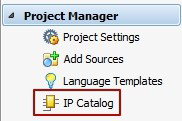
\includegraphics[width=0.6\textwidth]{1}
\caption{Рис.1}
\label{1_label}
\end{figure}

\begin{figure}[H]
\centering
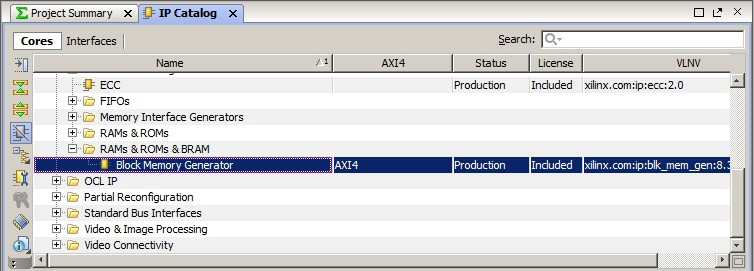
\includegraphics[width=0.6\textwidth]{2}
\caption{Рис.2}
\label{2_label}
\end{figure}

\subsection{Работа с интерфейсом BMG} 
Выбор типа и организации запоминающего устройства, формируемого на основе рассматриваемого параметризированного модуля, осуществляется с помощью соответствующего \emph {мастера} настройки параметров, который содержит от четырёх до шести (в зависимости от конфигурируемых параметров) диалоговых панелей.

\subsubsection{Basic}

\begin{figure}[h]
\centering
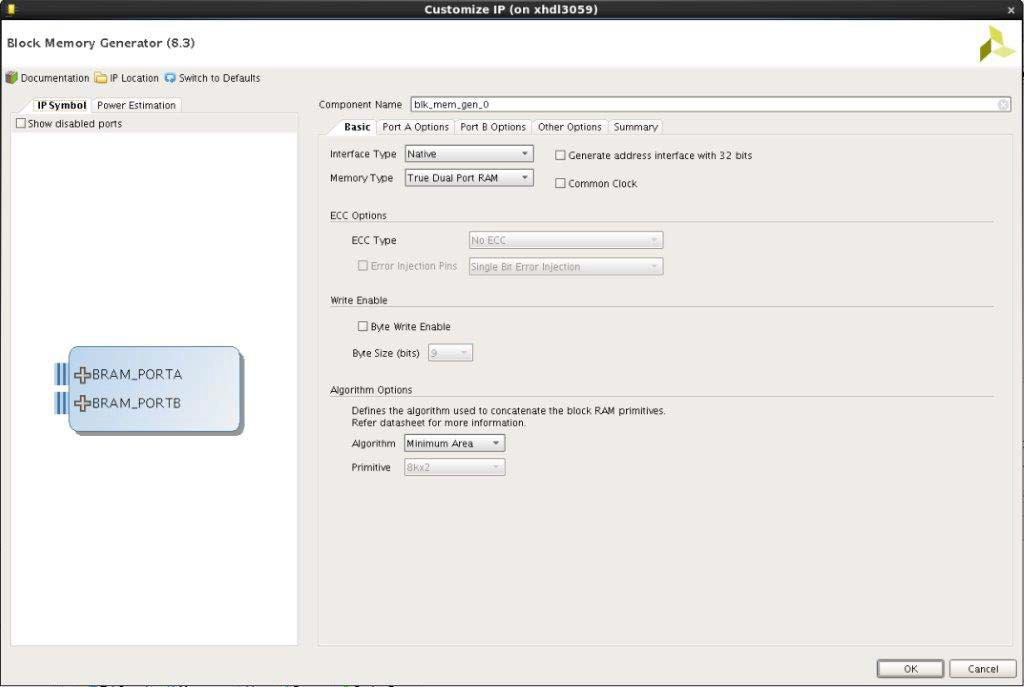
\includegraphics[width=0.6\textwidth]{3}
\caption{Рис.3}
\label{3_label}
\end{figure}

В стартовой диалоговой панели \emph {мастера}, вид которой показан на рисунке, указывается тип создаваемого элемента памяти, его название, а также алгоритм его реализации. 
\begin{itemize}
\item Название формируемого вида запоминающего устройства вводится с помощью клавиатуры в поле редактирования Component Name.
\end{itemize}

На выбор доступны два типа интерфейса – Native и AXI4.

Память блоков интерфейса AXI4 построена на памяти блоков нативного (Native) типа. Доступны два стиля интерфейса AXI4: AXI4 и AXI4-Lite. Также на выбор конфигурируется ядро. Далее на выбор предполагается настройка устройства памяти как ведомое или периферийно. В дополнение к приложениям, поддерживаемым нативным интерфейсом, AXI4 может также использоваться в приложениях AXI4 System Bus и приложениях типа Point-to-Point.

Для нативного типа интерфейса предполагаются следующие параметры настройки:

\begin{itemize}
\item Для определения типа генерируемого элемента памяти следует воспользоваться группой кнопок с зависимой фиксацией Memory Type. Если в нажатом состоянии зафиксирована кнопка Single Port RAM, то будет сформировано ОЗУ с одним портом записи и одним портом чтения данных. При нажатой кнопке Simple Dual Port RAM создается элемент двухпортовой оперативной памяти с одним портом чтения данных.Кроме того, при выборе данного типа памяти становится доступной опция ECC (Error Correction Checking) Type, созданная для регистрации и исправления ошибок с помощью кода Хэмминга и поиска необходимых совместимостей. Для генерации ОЗУ с двумя портами чтения и двумя портами записи данных нужно переключить в нажатое состояние кнопку True Dual Port RAM. Формирование однопортового постоянного запоминающего устройства осуществляется при нажатой кнопке Single Port ROM. Чтобы создать элемент двухпортовой постоянной памяти, следует перевести во включенное состояние кнопку Dual Port ROM. Для двухпортовых элементов доступна опция Common Clock для синхронизации часов ввода (управление одним буфером)
\item Также может быть установлен режим побайтной записи. Для этого нужно перевести в состояние \emph {включено} индикатор Use Byte Write Enable, который расположен во встроенной панели Write Enable.
\item Побайтная запись может осуществляться с контролем и без контроля четности. При этом размер записываемого байта (количество бит в байте) зависит от использования контроля четности. В случае отсутствия контроля четности длина байта составляет восемь бит. Чтобы побайтная запись выполнялась с контролем четности, в состав байта данных должно входить девять бит (восемь бит данных и один контрольный). 
\item Размер байта (и, соответственно, использование контроля четности) указывается с помощью поля выбора Byte Size.
\item Запоминающее устройство, генерируемое с помощью параметризированного модуля Block Memory Generator, строится в виде совокупности примитивов блочной памяти Block RAM primitive. В общем случае каждый из используемых примитивов может иметь различную организацию. Количество и состав возможных вариантов организации примитивов блочной памяти Block RAM primitive определяется выбранным семейством ПЛИС. Тип организации примитивов блочной памяти и алгоритм их соединения для получения запоминающего устройства с требуемой емкостью и организацией указывается с помощью двух кнопок с зависимой фиксацией, которые расположены во встроенной панели Algorithm. Когда в нажатом состоянии находится кнопка Minimum Area, создаваемый элемент памяти составляется из примитивов с различной организацией с целью минимизации используемого количества модулей блочной памяти Block RAM кристалла ПЛИС. При нажатой кнопке Low Power создаваемый элемент памяти будет состоять из тех же, модулей, что и в Minimum Area ядре, но включёнными только при записи или чтении. При нажатой кнопке Fixed Primitive для построения требуемого запоминающего устройства будут использоваться примитивы блочной памяти одного типа, организация которого указывается пользователем с помощью поля выбора Primitive. Содержимое выпадающего списка этого поля выбора зависит от семейства ПЛИС, для которого создается элемент памяти.
\end{itemize}


\subsubsection{Port A|B options}

Вторая диалоговая панель \emph{мастера} настройки параметров генератора оперативных и постоянных запоминающих устройств, реализуемых на основе блочной памяти ПЛИС, предназначена для определения емкости формируемого элемента памяти, а также описания организации и режима работы первого (или единственного) порта запоминающего устройства. 

\begin{figure}[h]
\centering
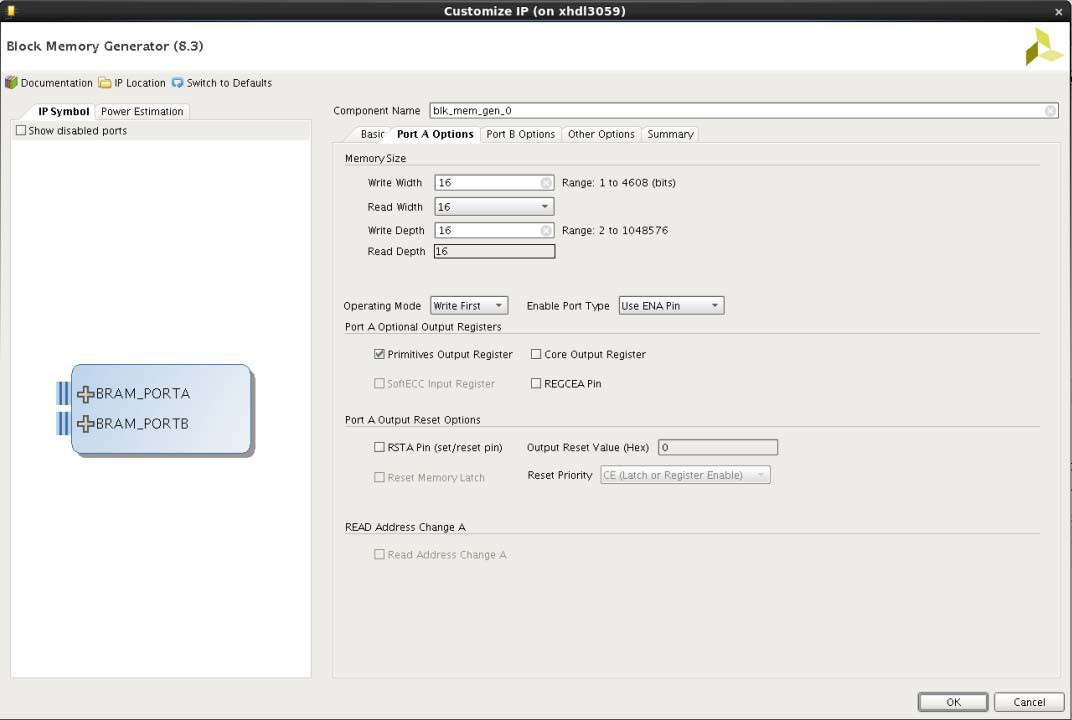
\includegraphics[width=0.6\textwidth]{4}
\caption{Рис.4}
\label{4_label}
\end{figure}

\begin{itemize}
\item Чтобы указать информационную емкость формируемого элемента памяти и разрядность первого (или единственного) порта записи и чтения данных, нужно воспользоваться полями редактирования и выбора, расположенными во встроенной панели Memory Size. Прежде всего, рекомендуется определить разрядность первого входного порта Port A, предназначенного для записи данных, с помощью поля редактирования Write Width. Требуемое число разрядов этого порта (в диапазоне от 1 до 1152) указывается с помощью клавиатуры, после активизации данного поля редактирования. Количество ячеек памяти в формируемом запоминающем устройстве задается в поле редактирования Write Depth. Максимальное значение этого параметра ограничено объемом физических ресурсов блочной памяти Block RAM используемого кристалла ПЛИС. Таким образом, информационная емкость создаваемого элемента памяти, выраженная в битах, равна произведению значений параметров Write Width и Write Depth. Разрядность первого (или единственного) выходного порта, используемого для чтения данных из памяти, определяется с помощью поля выбора Read Width. Выпадающий список этого поля выбора содержит допустимые варианты разрядности первого выходного порта, которые соответствуют установленному значению разрядности первого входного порта записи данных. Количество разрядов адреса (адресных входов) в формируемом запоминающем устройстве вычисляется автоматически, исходя из установленных значений параметров, рассмотренных выше. Значения параметров Write Width и Read Width должны быть кратны размеру байта данных, указанному в поле выбора Byte Size. В этом случае вместо обычного (одиночного) входа разрешения записи данных используется шина, количество разрядов которой вычисляется автоматически в соответствии с указанным значением разрядности порта записи. 
\item Для определения режима работы первого (или единственного) выходного порта элемента оперативной памяти, предназначенного для чтения данных, при выполнении операции записи данных в ОЗУ нужно воспользоваться группой кнопок с зависимой фиксацией Operating Mode. Если в нажатом состоянии находится кнопка Write First, то данные, поступающие во входной порт, записываются в соответствующую ячейку памяти (адрес которой задается комбинацией сигналов на адресных входах), после чего сразу передаются на выходы запоминающего устройства. При нажатии кнопки Read First в генерируемом элементе оперативной памяти будет установлен режим предварительного чтения данных из указанной ячейки перед записью новых данных в эту ячейку. Таким образом, при осуществлении операции записи данных, поступающих во входной порт формируемого элемента ОЗУ, на его выходах будет отображаться информация, которая содержалась в соответствующей ячейке перед этим (на предыдущем такте). Когда в нажатое состояние переводится кнопка No Change, в формируемом элементе ОЗУ будет установлен режим блокировки выходов при выполнении операции записи данных. В этом режиме на протяжении всего цикла записи выходы находятся в зафиксированном состоянии, которое соответствует последним считанным данным, присутствовавшим в момент переключения сигнала разрешения записи в активное состояние. 
\item Чтобы сформировать элемент запоминающего устройства с входом разрешения операций для первого порта, нужно переключить в нажатое состояние кнопку Use ENA Pin. При этом в созданном элементе памяти выполнение операций записи и чтения данных для первого порта будет возможно только при активном уровне сигнала на входе разрешения ENA.
\item Для определения состояния выходного регистра или защелки формируемого запоминающего устройства в режиме сброса (или установки) следует воспользоваться полем редактирования Output Reset Value (Hex), которое расположено во встроенной панели Output Reset. Значение, указываемое в этом поле редактирования, должно быть представлено в шестнадцатеричном формате. При этом количество шестнадцатеричных символов должно соответствовать разрядности первого порта чтения данных. Чтобы задействовать в формируемом элементе памяти вход синхронного сброса (или установки) для первого порта (Port A), следует установить индикатор Use SSRA Pin, находящийся в этой же встроенной панели, в состояние \emph {включено}. 
\item Если в стартовой диалоговой панели \emph {мастера} настройки параметров генератора элементов памяти был выбран двухпортовый тип запоминающего устройства, то третья диалоговая панель будет позволять определить основные параметры второго порта (Port B) создаваемого элемента памяти. Все параметры этого порта, за исключением разрядности, указываются так же, как и для первого порта (Port A). Количество разрядов второго порта записи данных не может быть установлено произвольно. Значение этого параметра должно быть кратным числу разрядов первого порта записи данных (с фиксированным набором коэффициентов кратности), которое было указано в диалоговой панели, представленной на рисунке. Поэтому разрядность второго порта записи данных задается с помощью поля выбора Write Width, выпадающий список которого содержит только допустимые значения данного параметра. Содержимое этого списка автоматически корректируется при изменении значения разрядности первого порта записи данных. 
\end{itemize}

\subsubsection{Other options}

Предпоследняя диалоговая панель \emph {мастера} настройки параметров генератора оперативных и постоянных запоминающих устройств, реализуемых на основе блочной памяти ПЛИС, позволяет выбрать тип и конфигурацию выходных регистров, а также указать параметры инициализации формируемого элемента памяти. 

\begin{figure}[h]
\centering
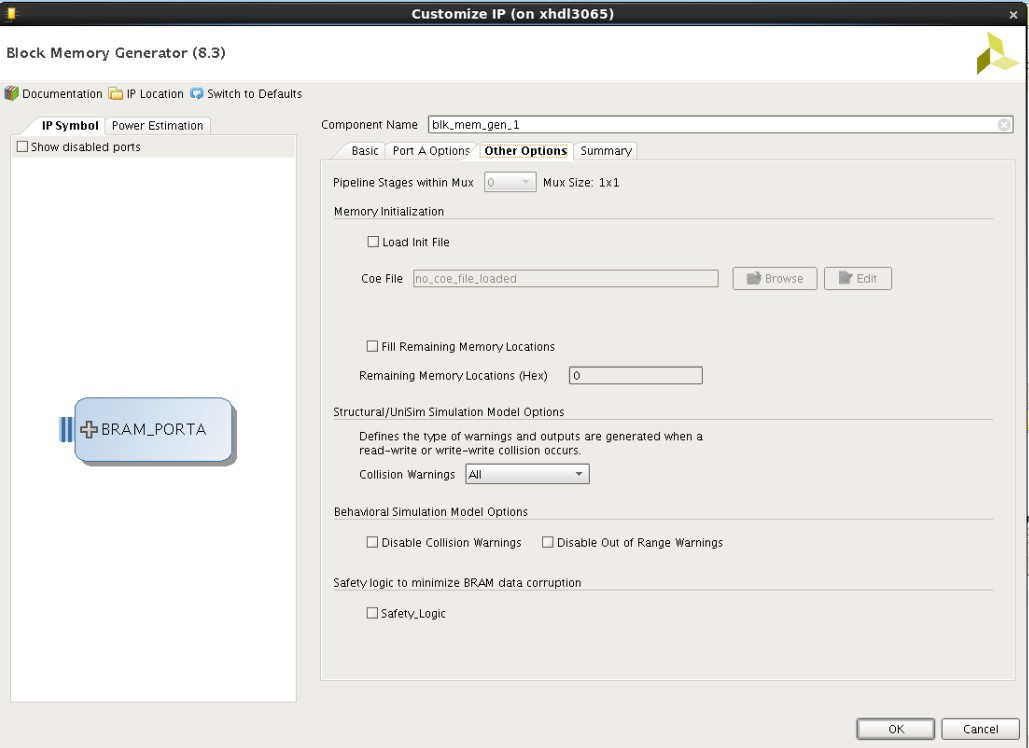
\includegraphics[width=0.6\textwidth]{5}
\caption{Рис.5}
\label{5_label}
\end{figure}

\begin{itemize}
\item Стадии конвейера в пределах Мультиплексора: доступна только, когда опция Register Output of Memory Core выбрана и для порта A и для порта B и когда у созданной памяти есть больше чем один примитив (так, чтобы MUX был необходим при выводе). Выберите значение 0, 1, 2, или 3 из выпадающего списка.
\item Для автоматической инициализации содержимого генерируемых запоминающих устройств, реализуемых на основе блочной памяти ПЛИС, следует определить значения соответствующих параметров с помощью элементов управления, которые расположены во встроенной панели Memory Initialization. Информацию, которую нужно записать в соответствующие ячейки формируемого элемента памяти, можно указать в виде файла формата COE. Для этого нужно, прежде всего, переключить индикатор Load Init File в состояние «включено», после чего станут доступными поле редактирования COE File и кнопка Browse. При нажатии на данную кнопку на экран выводится стандартная панель диалога открытия файла, с помощью которой нужно найти на одном из дисков компьютера требуемый файл, описывающий содержимое создаваемого запоминающего устройства. После выбора соответствующего файла и закрытия стандартной диалоговой панели его название автоматически отображается в поле редактирования COE File. Можно также с помощью клавиатуры сразу указать в этом поле редактирования название требуемого файла инициализации, не выполняя процедуру его поиска. Для быстрого просмотра содержимого выбранного файла нужно воспользоваться кнопкой Show, которая находится во встроенной панели Memory Initialization. Если указываемый файл инициализации описывает содержимое только части генерируемого запоминающего устройства, то все оставшиеся неинициализированными ячейки памяти могут быть заполнены по умолчанию значением, определяемым пользователем. С этой целью нужно установить индикатор Fill Remaining Memory Locations в состояние \emph {включено}. При этом становится доступным поле редактирования Remaining Memory Locations (Hex), в котором нужно с помощью клавиатуры указать шестнадцатеричное значение, записываемое по умолчанию в ячейки памяти, оставшиеся неопределенными. Количество шестнадцатеричных символов, указываемых в этом поле редактирования, должно соответствовать разрядности первого порта записи генерируемого запоминающего устройства. 
\item Structural/UNISIM Simulation Model Options: Выберите тип предупреждающих сообщений и выводов, сгенерированных структурной моделью моделирования в случае коллизий. Для опций ALL, WARNING ONLY и GENERATE X ONLY, обнаружения коллизий, опция активирована в моделях UNISIM, чтобы обработать коллизию при любом условии.
\item Behavioral Simulation Model Options: Выберите тип предупреждающих сообщений, сгенерированных моделью моделирования на поведенческом уровне. Выберите, должна ли модель принять синхронные часы (Общие Часы) для предупреждений коллизии.
\item Dynamic Power Saving: экономия электроэнергии включена в положении, когда память активно не используется в течение длительного периода времени. Если матрица элементов памяти входит в режим ожидания, данные сохраняются. Чтобы использовать память, установите контакт сна в 0.
\end{itemize}

\subsubsection{Summary}

Заключительная диалоговая панель \emph {мастера} настройки генератора оперативных и постоянных запоминающих устройств, реализуемых на основе блочной памяти ПЛИС, отражает параметры создаваемого устройства в виде списка.

\begin{figure}[h]
\centering
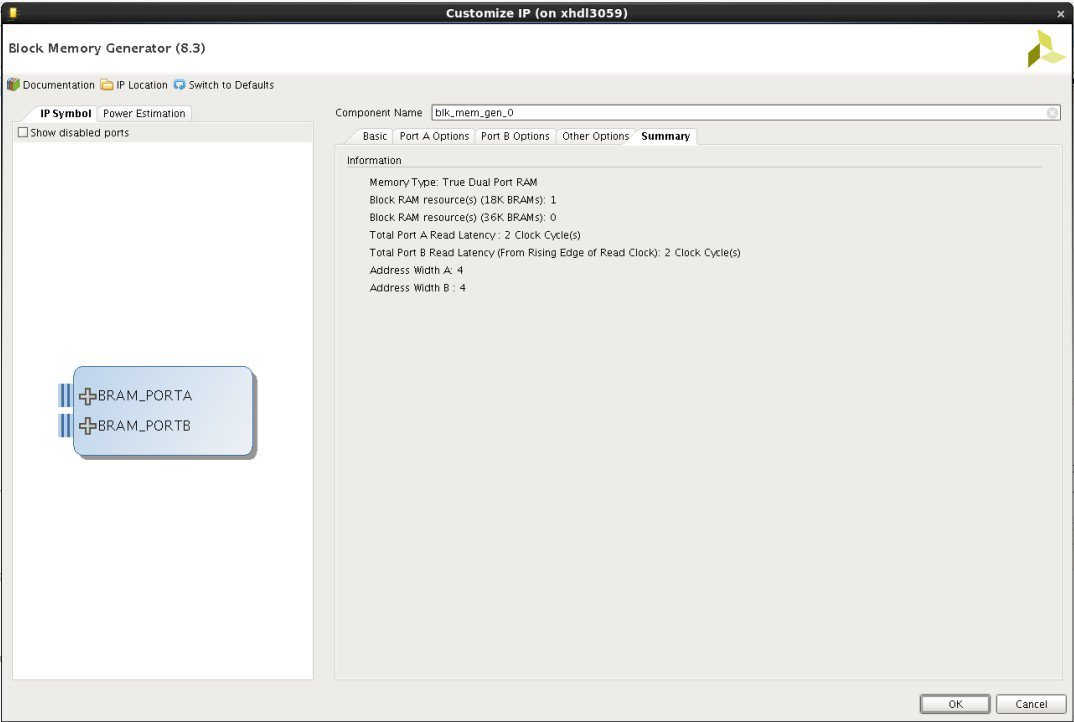
\includegraphics[width=0.6\textwidth]{6}
\caption{Рис.6}
\label{6_label}
\end{figure}

\begin{itemize}
\item Memory Type: Сообщает о выбранном типе памяти.
\item Block RAM Resources: Сообщает точный номер 18 K и 36 K блочных примитивов RAM, которые используются, чтобы создать ядро.
\item Total Port A Read Latency: номер тактов для Операции чтения для порта A. Этим значением управляют дополнительные выходные опции регистров для порта на предыдущей вкладке.
\item Total Port B Read Latency: номер тактов для Операции чтения для порта B. Этим значением управляют дополнительные выходные опции регистров для порта B на предыдущей вкладке.
\item Address Width: фактическая ширина адресной шины к каждому порту.
\end{itemize}

\subsubsection{Power Estimation}

\begin{figure}[h]
\centering
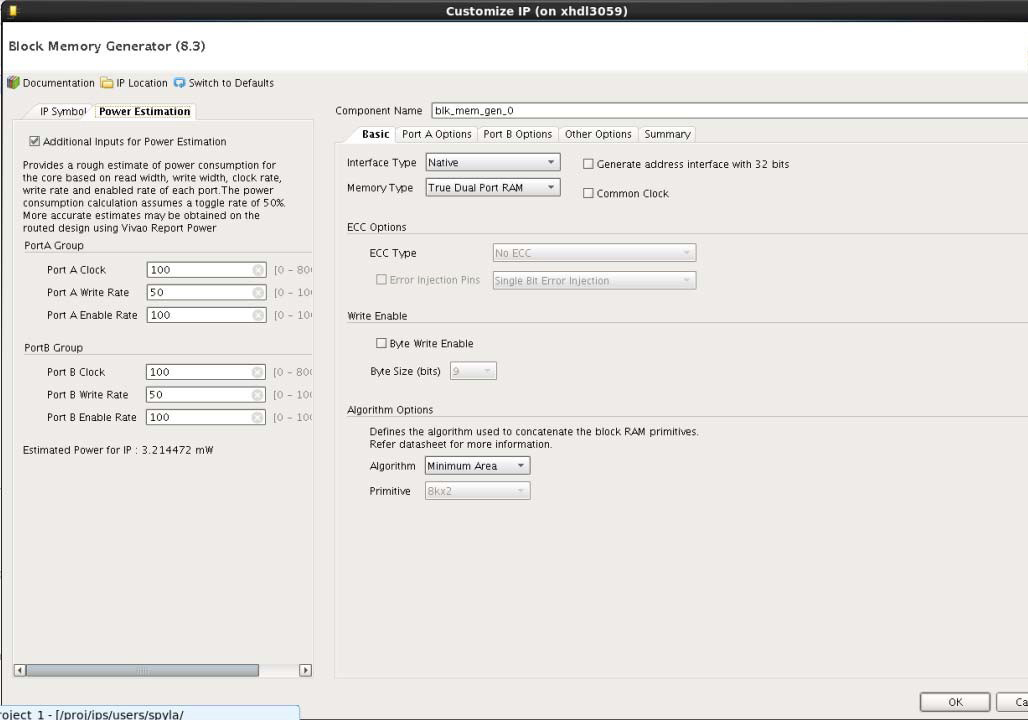
\includegraphics[width=0.6\textwidth]{7}
\caption{Рис.7}
\label{7_label}
\end{figure}

Вкладка Power Estimation на левой стороне IDE Vivado, показанная на рисунке, обеспечивает грубую оценку потребляемой мощности для ядра, основанного на сконфигурированных параметрах Read width, Write width, clock rate, Write rate and enable rate для каждого порта.
 
У этой вкладки есть опция  \emph {Additional Inputs for Power Estimation}, созданная для ввода дополнительных оценок потребляемой мощности. Можно ввести следующие параметры для расчета питания: Clock Frequency [A|B] (тактовая частота портов А и В), Write Rate [A|B] (скорость записи для портов А и В), Enable Rate [A|B] (средняя скорость доступа к портам А и В)

\subsection{Включение созданного ядра в код VHDL}

После выбора необходимых параметров для модуля BRAM следует нажать OK, a затем Generate во всплывающем окне. После того, как завершится синтез нашего модуля, переходим на вкладку IP Sources и открываем Файл в формате .vho в папке Instantiation Template(см. Рис. 8)

\begin{figure}[h]
\centering
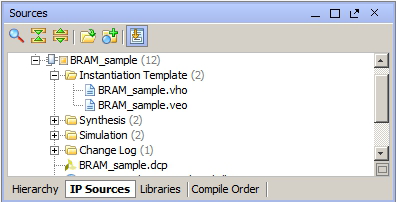
\includegraphics[width=0.6\textwidth]{8}
\caption{Рис. 8}
\label{8_label}
\end{figure}

В этом файле уже созданы вставки для определения компонента в основном коде и инстанциация для тестбенча (рис. 9-10)

\begin{figure}[h]
\centering
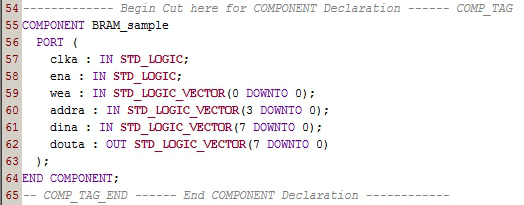
\includegraphics[width=0.6\textwidth]{9}
\caption{Рис. 9}
\label{9_label}
\end{figure}

\begin{figure}[h]
\centering
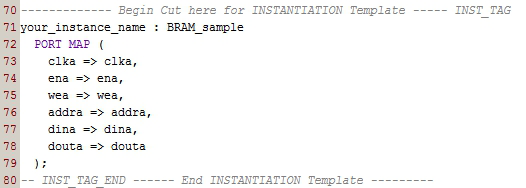
\includegraphics[width=0.6\textwidth]{10}
\caption{Рис. 10}
\label{10_label}
\end{figure}

\subsection{Симуляция}

В качестве примера рассмотрим BRAM со следующими параметрами (всё, что не указано ~-- по умолчанию):
\begin{enumerate}
%\item Component Name: BRAM_sample, Algorithm: Low Power
\item Algorithm: Low Power
\item Write width:8, Read width:8, Write depth:16
\item Галочка Fill Remaining memory locations
\end{enumerate}

Напишем тестбенч для данного модуля памяти: 

\lstinputlisting[caption=Тестбенч, label=09-bram]{proga1.vhd}

Результаты симуляции:

\begin{figure}[h]
\centering
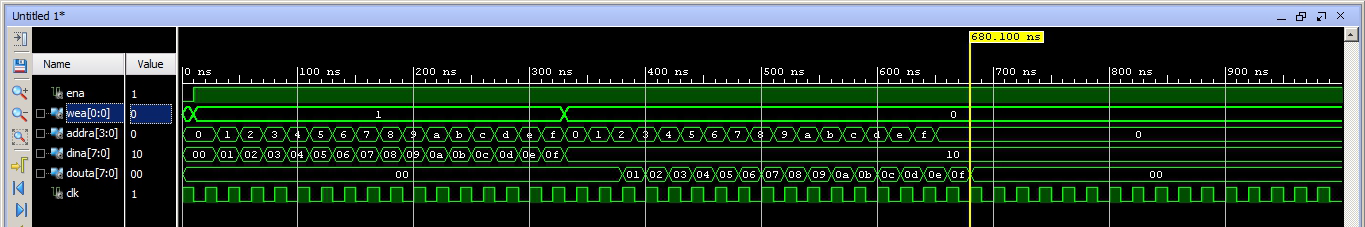
\includegraphics[width=0.6\textwidth]{11}
\caption{Рис. 11}
\label{11_label}
\end{figure}

\section{Лабораторная работа: Накопитель памяти на основе BRAM}

Задача: написать VHDL-код накопителя, использующего BRAM. Накопитель имеет вход $data(din)$ и вход $valid(dv_in)$, в накопитель поступают данные с паузами; затем, когда поступило N (16) отсчетов данных, буфер выдает последовательно без пауз все пришедшие ранее отсчеты данных.

\subsection{Создаём модуль BRAM}
\subsection{Реализация на VHDL}

\lstinputlisting[caption=Реализация кода, label=09-bram]{proga2.vhd}

\subsection{Самопроверяющийся тестбенч}

\lstinputlisting[caption=Тестбенч, label=09-bram]{proga3.vhd}
\chapter{Работа с очередями FIFO}

\emph{Интерфес FIFO. Асинхронных режим. Режимы работы FIFO: Standard и First Word Fall Through. Интерфейс AXI Stream.}

\section{Содержание главы}

Основной литературой по FIFO является PG057. Требуется:
\begin{itemize}
\item описать всю последовательность действий по созданию и кастомизации ядра FIFO, а также включению его в код на VHDL, сделав при этом упор на интерфейс \emph{Native} и на интерфейс \emph{AXI4-Stream} (про интерфейс AXI4 Memory Mapped достаточно упомянуть);
\item написать testbench для ядра FIFO, чтобы показать его функциональность (т.е. то, как ядро работает), привести пример временных форм сигналов из симулятора;
\item описать принцип работы FIFO (описать два указателя~-- на начало и конец очереди в памяти, когда и как они увеличиваются и т.д.);
\item написать, отладить и описать VHDL-код усредняющего FIFO. Обязателен testbench.
\end{itemize}

\section{Оформление}

Очень хорошее и краткое введение в LaTeX можно найти в книге Столярова (\href{url}{http://www.stolyarov.info/books/latex3days/}).

\section{Заголовок 1-го уровня}
\subsection{Заголовок 2-го уровня}
\subsubsection{Заголовок 3-го уровня}

Текст. Текст. Текст. \emph{Текст курсивом.} Поставить тире~-- вот так. Текст в "<кавычках">.

Чтобы сделать новый абзац, нужно пропустить строку.

Пример кода:

\begin{Code}
\begin{lstlisting}
library IEEE;
use IEEE.STD_LOGIC_1164.ALL;

entity Latch is
    port ( C : in  STD_LOGIC;
           D : in  STD_LOGIC;
           Q : out STD_LOGIC);
end Latch;

architecture Behavioral of Latch is
    signal q_tmp : std_logic := '0';
begin
    latch_process: process (C, D)
    begin
        if (C = '1') then
            q_tmp <= D;
        end if;
    end process;
    Q <= q_tmp;
end Behavioral;
\end{lstlisting}
\end{Code}

Пример кода в строке: \lstinline?С = 1?. Или вот так: \lstinline?S(7 downto 1) <= S(6 downto 0);?. Здесь код помещен между знаками вопроса.

Пример нумерованного списка:

\begin{enumerate}
\item Пункт 1.
\item Пункт 2.
\item Пункт 3.
\end{enumerate}

Пример ненумерованного списка:

\begin{itemize}
\item Пункт 1.
\item Пункт 2.
\item Пункт 3.
\end{itemize}

Вот так оформляется таблица с тремя колонками:

\begin{table}[h]
\centering
\begin{tabular}{|c|c|c|}
\hline
input               & \multicolumn{2}{c|}{output} \\ \hline
r                   & code        & active         \\ \hline
\texttt{1{-}{-}{-}} & \texttt{11} & \texttt{1}     \\
\texttt{01{-}{-}}   & \texttt{10} & \texttt{1}     \\
\texttt{001-}       & \texttt{01} & \texttt{1}     \\
\texttt{0001}       & \texttt{00} & \texttt{1}     \\
\texttt{0000}       & \texttt{00} & \texttt{0}     \\
\hline
\end{tabular}
\end{table}

Рисование осуществляется с помощью пакета 'TikZ':

\begin{figure}[ht]
\centering
\begin{tikzpicture}[>=latex']
\tikzstyle{arith_op} = [draw, fill=blue!20, circle, minimum size=2em]

% inputs
\node at (0,4) (input_a) {\texttt{a}};
\node at (0,3) (input_b) {\texttt{b}};
\node at (0,1) (input_c) {\texttt{c}};
\node at (0,0) (input_1) {\texttt{1}};

% operations
\node[arith_op] at (1,3) (block_plus_1) {$+$};
\node[arith_op] at (1,1) (block_plus_2) {$+$};
\node[arith_op] at (2,2) (block_minus) {$-$};

% connections
\draw[->] (input_a) -- (1,4) -- node {} (block_plus_1);
\draw[->] (input_b) -- node {} (block_plus_1);
\draw[->] (input_c) -- node {} (block_plus_2);
\draw[->] (input_1) -- (1,0) -- node {} (block_plus_2);
\draw[->] (block_plus_1) -- (2,3) -- node {} (block_minus);
\draw[->] (block_plus_2) -- (2,1) -- node {} (block_minus);
\draw[->] (block_minus) -- (3,2);
\end{tikzpicture}
\caption{Оптимизированная комбинационная схема.}
\label{label_fig_1}
\end{figure}

Ссылка на рисунок делается по \emph{label} вот так: \ref{label_fig_1}.

Вставка скриншотов программ (PNG) возможна следующим образом (файл изображения находится в папке с кодом):

\begin{figure}[h]
\centering
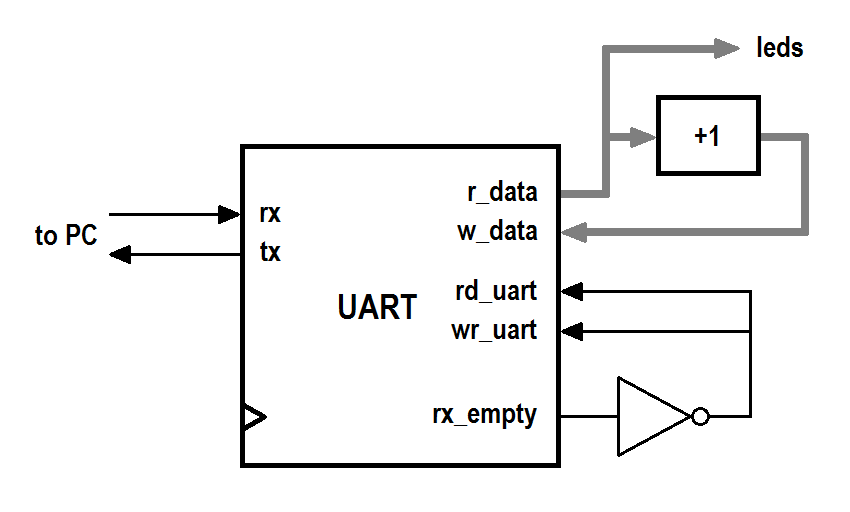
\includegraphics[width=0.6\textwidth]{test_fig}
\caption{Некий рисунок}
\label{test_fig_label}
\end{figure}
\chapter{Передача данных через UART}

\emph{Описание протокола, реализация в ПЛИС}

\section{Вывод на консоль во время симуляции}

\chapter{Отладка проекта в железе}

\emph{Описание работы Debug Core}

\section{Вывод на консоль во время симуляции}


\end{document}
